\chapter{Обзор предметной области}
\label{chap:overview}

\section{Модели случайных графов}
\label{sec:random_graph_models}

\subsection{Классическая модель Эрдеша–Реньи}
\label{subsec:erdos_renyi}

Классическая модель случайного графа Эрдеша–Реньи представляет собой вероятностную модель неориентированного графа на $n$ вершинах~\cite{Erdos1959}. 
Существуют две эквивалентные версии модели. 
В модели $G(n, M)$ выбирается равновероятно один из всех графов с фиксированным числом вершин $n$ и ровно $M$ рёбрами.
В более распространённой \textit{биномиальной} модели $G(n, p)$ предполагается, что каждый из $\binom{n}{2}$ возможных ребёр присутствует независимо с вероятностью $p$.

Модели Эрдеша–Реньи заложили основу теории случайных графов и вероятностного метода в комбинаторике.
При больших $n$ такие графы демонстрируют резкие \textit{пороговые явления}: многие свойства графа возникают почти наверняка, как только параметр $p$ превышает некоторый критический порог (зависящий от $n$).
Например, для достаточно малых $p$ граф почти наверняка несвязен и разбит на множество мелких компонент, но при увеличении $p$ происходит фазовый переход к связному графу.
Ниже рассмотрен классический пример такого перехода – появление гигантской компоненты.

\subsection{Порог появления гигантской компоненты}
\label{subsec:giant_component_threshold}

Одним из самых известных результатов Эрдеша–Реньи является порог появления гигантской связной компоненты в случайном графе.
Под гигантской компонентой понимают связную компоненту размера порядка $n$ (то есть содержащую положительную долю всех вершин графа).
Для модели $G(n,p)$ при $n \to \infty$ существует критическое значение $p_c \sim \frac{1}{n}$, при превышении которого в графе почти наверняка присутствует единственная гигантская компонента. 
Точнее, если $p = \frac{c}{n}$, то наблюдается фазовый переход при $c=1$.
Когда $c < 1$ (то есть $p < \frac{1}{n}$), случайный граф со стремящейся к 1 вероятностью состоит лишь из множества малых компонент (размер каждой не более $O(\ln n)$).
При $c > 1$ ($p > \frac{1}{n}$) почти наверняка возникает единственная большая компонента, содержащая $\Theta(n)$ вершин, тогда как все остальные компоненты остаются малыми.
В точке $p \approx \frac{1}{n}$ происходит переходный режим: максимальная компонента имеет размер порядка $n^{2/3}$.
Это явление аналогично перколяционному переходу в статистической физике; порог $p_c = 1/n$ часто называют критической точкой перколяции на полном графе.

Данный результат был впервые доказан Эрдешем и Реньи~\cite{Erdos1959}.
Он иллюстрирует свойственный случайным графам эффект: небольшое стохастическое изменение параметров (от $p = \frac{1-\varepsilon}{n}$ к $p = \frac{1+\varepsilon}{n}$) приводит к резкому структурному изменению графа (появлению «гиганта»).
В дальнейшем мы увидим аналогичные идеи при рассмотрении разбиения генома на фрагменты под действием случайных перестроек: там также наблюдается переход от сохранения большой цельной части структуры к её фрагментации на множество небольших блоков.

\subsection{Аффинные модификации модели случайных графов}
\label{subsec:affine_modifications}

Классическая модель Эрдеша–Реньи предполагает однородность: все вершины и потенциальные рёбра статистически эквивалентны, вероятность появления любого ребра одинакова ($p$) и независима от других.
Однако во многих реальных сетях (и тем более в структурных моделях геномов) такая простая случайность не соблюдается — некоторые связи возникают чаще других, степень вершин может подчиняться неоднородному распределению, наблюдается кластеризация и пр. Поэтому были предложены многочисленные обобщения модели случайного графа, вводящие \textit{неоднородности} в вероятность ребер. Условно такие обобщения можно назвать «аффинными» модификациями модели, поскольку они сохраняют линейный характер зависимости вероятностей от некоторых параметров (например, от свойств вершин или уже существующих степеней), но отходят от строгой равновероятности всех связей.

Одним из направлений обобщения являются модели с заданной степенной последовательностью.
В работе Ньюмана, Строгaтза и Уоттса~\cite{Newman2001} предложена генеративная модель случайного графа с произвольным заданным распределением степеней вершнин.
В ней каждой вершине заранее приписывается случайная степень (например, согласно некоторому распределению), а затем вершины случайно спариваются по полурёбрам (англ. \textit{half-edges}) до достижения требуемых степеней.
Эта модель эквивалентна так называемой конфигурационной модели и позволяет получать случайные графы с заданными свойствами (например, с тяжёлыми хвостами распределения степеней), что является аффинной модификацией по отношению к модели Эрдеша–Реньи (где распределение степеней, напротив, близко к пуассоновскому и быстро убывает).

Другая известная модификация — модель предпочтительного присоединения (модель Барабаши — Альберт)~\cite{Barabasi1999}. 
В ней граф строится динамически: вершины добавляются последовательно, и каждая новая вершина соединяется с некоторым числом ранее добавленных вершин с вероятностями, пропорциональными степеням этих существующих вершин. 
Таким образом, вероятность образования нового ребра линейно (``аффинно'') зависит от текущей степени вершины: $\Pr(\text{новое ребро соединится с вершиной } i) \propto k_i + c$, где $k_i$ — степень вершины $i$, а $c$ — некоторая константа предпочтения.
Данная модель генерирует ``безмасштабные'' сети с степенным распределением степеней вершин, что значительно отличает её от модели Эрдеша–Реньи. 

Существуют и геометрические (пространственные) случайные графы, в которых вершины имеют случайные координаты, и рёбра возникают с вероятностью, зависящей от расстояния между вершинами (например, модель единичного диска).
Это также вводит ``аффинность'' через функцию расстояния: близкие вершины имеют повышенный шанс связаться. 

Обобщения модели случайного графа важны тем, что позволяют более адекватно моделировать сложные системы.
В частности, при моделировании эволюции геномов нам потребуется учитывать неоднородности в вероятностях «сопряжённости» элементов генома (некоторые элементы чаще участвуют в эволюционных событиях, чем другие).
Это является прямым аналогом отхода от простейшей равномерной случайности, подобно переходу от $G(n,p)$ к моделям с ``горячими точками'' (hot spots) или с индивидуальными вероятностями для различных потенциальных связей.
Далее мы увидим, как такое введение ``весов'' и неоднородностей применяется к специальному графу, моделирующему структуры генома.

\subsection{Граф точек разрыва и его модификации}
\label{subsec:breakpoint_graph}

При сравнении двух геномов, подвергшихся перестройкам, удобным формализмом является граф точек разрыва (англ. \textit{breakpoint graph}).
Этот граф строится следующим образом.
Сначала геномы представляют в виде последовательностей идентифицируемых фрагментов (блоков синтении) с учётом ориентации.
Вершинами графа служат концы этих блоков (точки разрыва между блоками).
Далее для каждого генома проводится соединение концов блоков, следующих друг за другом в данном геноме, при помощи рёбер (то есть каждое \textit{соседство} двух блоков в геноме даёт ребро в графе).
Таким образом, если сравниваются два генома $P$ и $Q$, то в граф добавляются рёбра двух типов: рёбра типа $P$ (отражающие соседства в первом геноме) и рёбра типа $Q$ (соседства во втором геноме).
В итоге получается 2-расцветочный мультиграф с $2n$ вершинами (если в обоих геномах $n$ блоков) и, в общем случае, $2n$ рёбрами (по $n$ рёбер каждого типа, если считать, что каждый геном однокрохромосомный без разрывов).
Каждый узел этого графа имеет степень 2 (по одному ребру от каждого генома), поэтому компоненты графа образуют циклы различной длины. 

Количество циклов в графе точек разрыва тесно связано с расстоянием между геномами в перестройках.
В частности, для моделей без дупликаций справедливо, что чем больше циклов, тем ближе геномы.
Например, в случае одной хромосомы без разрывов (то есть геномы представимы как перестановки), расстояние в операциях DCJ можно вычислить как $d_{\text{DCJ}} = n - c$, где $n$ — число блоков, а $c$ — количество циклов в объединённом графе.
Интуитивно это означает: каждый цикл свидетельствует о том, что соответствующие элементы уже находятся на «правильных местах» друг относительно друга, и не требуют дополнительных операций для преобразования одного генома в другой; оставшиеся несовпадения требуют операций перестройки.
Таким образом, граф точек разрыва служит ключевым инструментом для вычисления минимального числа необходимых операций, т.е. расстояния перестройки между двумя геномами.

Модель случайных перестроек генома часто предполагает, что разрывы в геноме происходят случайно.
Если предположить, что каждый возможный разрыв (точка между геномными элементами) с равной вероятностью участвует в каждой операции перестройки, то граф точек разрыва между геномами после $k$ случайных операций будет обладать статистическими свойствами, близкими к свойствам случайного графа.
Например, при достаточном числе перестроек можно ожидать, что большинство циклов будут короткими (2 или 4 вершины), и лишь немногие компоненты свяжут значительную часть вершин графа (аналогия с гигантской компонентой) — иначе говоря, исходный порядок блоков будет почти полностью ``перемешан''.
Однако реальные эволюционные процессы могут отличаться от простого равномерного случайного разрыва: существуют области генома, более устойчивые к перестройкам, и наоборот, участки, ломкие и перестраивающиеся неоднократно.
Это приводит к модификациям классического графа разрывов, в которые включаются \textit{веса} или дополнительные параметры, отражающие неоднородность генома.

Однако стандартный граф точек разрыва не учитывает неоднородность генома: все разрывы считаются равновероятными.
В реальных биологических данных некоторые области генома склонны к частым перестройкам (т.\,н. хрупкие регионы), тогда как другие остаются стабильными.
Чтобы учесть эту особенность, вводится модифицированный граф точек разрыва с весами.
В таком графе каждому ребру (точке разрыва) приписывается вес, отражающий вероятность или частоту взаимодействия именно в этом месте~\cite{tannier2016}.
Весовая схема может быть основана на эмпирических данных или результатах предварительного статистического анализа геномных перестроек.

Другой модификацией является построение мульти-графа разрывов (англ. \textit{breakpoint multigraph}) для множества геномов.
Если имеется коллекция близкородственных геномов (например, виды или штаммы бактерий), можно обобщить граф разрывов на несколько геномов: вершины по-прежнему соответствуют концам блоков, а рёбра добавляются для \emph{каждого} генома из коллекции, отражая соседства блоков в этом геноме.
При этом каждое ребро помечается меткой, указывающей, какому геному (или листу филогенетического дерева) оно принадлежит.
В результате между двумя вершинами может быть несколько рёбер (по одному от некоторых геномов) — так формируются консенсусные мульти-рёбра (англ. \textit{consensus multi-edge}), отражающие тот факт, что несколько геномов имеют одинаковое соседство блоков.
Такой мультиграф позволяет одновременно анализировать сходства и различия в упорядочении блоков у всех рассматриваемых видов
Более того, он служит основой для выявления эволюционных событий: разрывы (отсутствие определённого соседства у части видов) и перестройки (например, наличие 4-цикла, свидетельствующего об инверсии в некоторых геномах).
В следующем разделе будет показано, как на базе мультиграфа разрывов можно формализовать признаки (англ. \textit{characters}) и идентифицировать параллельные изменения, сравнивая распределение этих признаков на филогенетическом дереве.

\section{Постановка задачи оценки расстояний между структурами}
\label{sec:distance_estimation}

\subsection{Опеределение шага процесса}
\label{subsec:dcj_operation}

Операция двойной разрез и слияние (англ. \textit{DCJ, Double Cut and Join}) является ключевым понятием в моделировании эволюционных перестроек геномов.
Данная операция формализует различные типы реальных перестроек, таких как инверсии, транслокации, слияния и разрывы хромосом, посредством единой математической операции~\cite{yancopoulos2005}.
В терминах графа точек разрыва, каждая операция двойной разрез и слияние соответствует изменению структуры рёбер графа, которые отражают взаимное расположение геномных фрагментов.

Формально, операция двойной разрез и слияние выполняется следующим образом:
\begin{enumerate}
    \item Выбираются два ребра (или теломерные вершины) графа.
    \item Оба выбранных ребра разрезаются, образуя четыре свободных конца.
    \item Затем эти концы соединяются заново одним из возможных способов, который отличается от исходного состояния.
\end{enumerate}

В зависимости от выбора исходных рёбер, операция двойной разрез и слияние может иметь несколько исходов:
\begin{itemize}
    \item Если выбираются два ребра из одного и того же цикла или пути, то двойной разрез и слияние может разделить его на два меньших цикла или пути.
    \item Если выбираются рёбра из разных циклов или путей, то двойной разрез и слияние может привести к их слиянию.
    \item Если выбирается теломерная вершина, операция может привести к преобразованию линейной хромосомы в циклическую или наоборот.
\end{itemize}

В случае модифицированного графа точек разрыва, в котором рёбра имеют веса, операция двойной разрез и слияние применяется аналогичным образом, однако вероятность выбора тех или иных рёбер теперь определяется их весами. 
Конкретно, пары рёбер выбираются с вероятностью, пропорциональной произведению их весов.
После выполнения операции DCJ, веса вновь образованных рёбер пересчитываются согласно заданным правилам модели, таким образом отражая изменение состояния генома и перераспределение вероятностей будущих перестроек.

Использование весового подхода в операции двойной разрез и слияние позволяет более точно отражать реальные биологические процессы, в частности учитывая неоднородность геномов по склонности к перестройкам, что существенно повышает точность оценки эволюционного расстояния между структурами.

\subsection{Метрика минимального числа операций}
\label{sec:minimal_operations}

Для количественной оценки эволюционных различий между двумя геномными структурами обычно вводится понятие расстояния, основанного на числе эволюционных событий.
Парсимониальное расстояние определяется как минимальное число определённых операций перестройки, необходимое для превращения одной геномной последовательности в другую.
Таким образом, расстояние в метрике двойной разрез и склеивание даёт наименьшее число разрезов/слияний, требуемых для преобразования одного генома в другой.

Расстояние, определённое как минимум операций (иногда его называют парсимониальное расстояние), широко используется благодаря вычислительной простоте во многих случаях.
Для бездупликатных геномов парсимониальное расстояние вычисляется напрямую из графа разрывов, как отмечалось выше.
В более простых случаях монохромосомных геномов без инверсий расстояние сводится к подсчёту количества циклов в графе.
Во всех этих случаях такое расстояние действительно является метрикой на множестве геномных последовательностей.

Однако метрика минимальных операций адекватна эволюционному расстоянию лишь при условии небольшого числа различий.
Для близкородственных геномов, которые эволюционировали от общего предка посредством относительно малого числа перестроек, минимальное число операций практически совпадает с истинным числом событий (поскольку маловероятны сложные случаи, когда несколько перестроек ``компенсируют'' друг друга).
Но в случае отдалённых геномов (существенно расходившихся длительное время) парсимонианское расстояние становится ненадёжным: оно, как правило, занижает реальное число произошедших перестроек.
Это связано с тем, что при значительном эволюционном расстоянии многие перестройки могут накладываться, повторно ломать уже однажды разорванные места или независимо затрагивать одни и те же области.
В результате две сильно перестроенные геномные последовательности могут казаться ближе (в терминах минимальных операций), чем это было бы по факту эволюции.
Например, если какой-то участок хромосомы переворачивался несколько, финальное сравнение покажет либо одно изменение, либо вообще отсутствие отличий (если вернулся исходный порядок), тогда как реально событий было больше одного.

\subsection{Вероятностная модель поломки случайных регионов}
\label{subsec:random_breakage}

Одним из основных вероятностных подходов к моделированию эволюции генома является модель случайных разрывов (англ \textit{Random Breakage Model, RBM})~\cite{Lin2008}.
В рамках этой модели предполагается, что у генома нет предпочтительных мест для перестроек: каждое возможное место разрыва равновероятно может участвовать в перестройке, и события разрыва происходят независимо друг от друга.
Иными словами, не существует \textit{горячих точек} хромосомных перестроек, и распределение точек разрыва по геному однородно.
Данная гипотеза восходит к работе Nadeau and Taylor (1984), в которой анализировалась длина сохранившихся сегментов между видами.
Выводы указали, что распределение размеров синтенных блоков соответствует случайному (показательному) распределению разрывов, что подтвердило модель случайных поломок на том этапе исследований.

Модель случайных разрывов можно переформулировать на языке случайных графов: если представить каждый потенциальный разрыв (между двумя соседними основаниями генома или между блоками) как ``ребро'' между сегментами, то каждая перестройка соответствует случайному выбору такого ребра.
За длительное эволюционное время множество перестроек приведёт к тому, что геном дробится на сегменты, и процесс можно уподобить случайному разбиению отрезка на части.
Предсказания данной модели включают, например, экспоненциальное распределение размеров оставшихся цельных сегментов генома и линейную зависимость количества разрывов от эволюционного времени.

Однако последующие исследования поставили под сомнение универсальность модели случайных разрывов.
В начале 2000-х с накоплением сравнительных данных по полным геномам было обнаружено, что разрывы далеко не всегда распределены равномерно: напротив, некоторые области генома разных видов совпадают по расположению точек разрыва гораздо чаще, чем ожидалось случайно.
Так, Певзнер и Теслер~\cite{Pevzner03} при сравнении геномов человека и мыши выявили кластеры повторно используемых точек разрыва, противоречащие модели случайных разрывов.
Они предположили существование хрупких (англ. \textit{fragile}) в геноме, более склонных к перестройкам, и сформулировали альтернативную гипотезу эволюции хромосом, получившую название модель хрупких разрывов (англ. \textit{fragile breakage model}).

Тем не менее, модель случайных разрывов остаётся важной нулевой моделью: она проста и позволяет выводить явные формулы.
Например, если геномы эволюционируют по этой модели, можно попытаться оценивать число перестроек на основе наблюдаемого числа разрывов и некоторых статистических гипотез.
Однако, как было отмечено выше, такая оценка будет систематически заниженной при наличии повторных разрывов в одних и тех же местах.
Для учета этого феномена нужны более сложные модели.

\subsection{Вероятностная модель поломки хрупких регионов}
\label{subsec:fragile_breakage}

Модель хрупких регионов (англ. \textit{Fragile Breakage Model, FBM}) была предложена для объяснения отклонений от случайного распределения разрывов.
В рамках FBM предполагается, что геном состоит из участков с различной хрупкостью: одни регионы могут многократно участвовать в перестройках (``хрупкие''), тогда как другие относительно устойчивы и разрываются редко (``устойчивые'').
Таким образом, перестройки происходят не в случайных местах, а преимущественно в определённых горячих точках (англ. \textit{hotspots}).
Модель хрупких регионов более сложна, чем модель случайных регионов, но она позволяет получать оценки числа перестроек с учётом наблюдаемого повторного использования разрывов.
Например, если в сравнении геномов выявлено меньше разрывов, чем ожидалось для данного числа операций, модель хрупких регионов объясняет это тем, что некоторые операции приходились на одни и те же места (``накладывались'').
Для количественной оценки эволюционной дистанции в таких условиях разрабатываются статистические методы, основанные на вероятностных характеристиках графа разрывов.
В частности, учитывается распределение циклов в графе разрывов: наличие необычно большого количества циклов определённых длин может свидетельствовать о неоднократных перестройках в одних и тех же местах.


Поставленная гипотеза получила развитие в количественных моделях: в частности, Танье и др.~\cite{tannier2016} предложили формализованную стохастическую модель эволюции, называемую INFER (англ. \textit{Inversion History with Fragile Regions}).
Хотя изначально INFER формулировалась для инверсий, она обобщается на любые операции эмулируемые с помощью двойного разреза и склеивания.

В модели INFER каждому потенциальному месту разрыва (каждому хрупкому региону и теломерам) приписывается вероятность $p_i$ быть задействованным в перестройке (причём $\sum_i p_i = 1$).
Эволюция генома моделируется как марковский процесс: на каждом шаге выбираются два места разрыва (скажем, $i$ и $j$) с вероятностями $p_i$ и $p_j$ соответственно, после чего выполняется операция DCJ, затрагивающая эти два места.
В результате образуются новые точки разрыва (например, если разрыв произошёл внутри региона, он разделяется на два новых региона), и вероятности ломкости обновляются для новых регионов по некоторому правилу.
В версии~\cite{tannier2016} используется правило равномерного ``разделения'' вероятностей: грубо говоря, вероятность $p_i$ разорванного региона распределяется между вновь образованными частями пропорционально случайным коэффициентам, чтобы их сумма равнялась $p_i$.
Это означает, что регион, однажды разорвавшийся, может частично сохранить высокую ломкость в одной из своих частей.
Несмотря на то, что в данной статье были предложена вероятностная модель более точно описывающая эволюцию генома, предложенные оценки являются лимитированными и выражены в виде бесконечных рядов.

Таким образом, использование вероятностных моделей и соответствующих статистических оценивателей позволяет более надёжно измерять расстояния между геномными структурами, что важно для построения корректных филогенетических гипотез и понимания механизмов эволюции.

\section{Методы анализа параллельных изменений в древовидных структурах}
\label{sec:dirichlet_model}

\subsection{Параллельные изменения как выпуклые признаки на деревьях}
\label{subsec:modified_dcj}

В филогенетике признак (англ. \textit{character}) называют выпуклым (англ. \textit{convex}) на данном эволюционном дереве, если множество видов (листьев), обладающих этим признаком, образует связное поддерево.
Эквивалентно, признак выпуклый (свободный от гомоплазии), если его можно объяснить одним появлением (или одним исчезновением) на некоторой ветви дерева~\ref{fig:convex-example-convex}.
В противном случае признак является невыпуслым (с гомоплазией), то есть его возникновение или утрата требуются в нескольких независимых точках дерева для согласования с наблюдаемым распределением~\ref{fig:convex-example-unconvex}.
В контексте геномных перестроек признаком может служить, например, наличие определённого геномного соседства или, напротив, факт разрыва между двумя геномными элементами.
Если такой признак выпуклый, это означает, что соответствующая перестройка произошла единожды у общего предка группы организмов.
Если же признак невыпуклый, значит похожие перестройки имели место неоднократно в разных филогенетических линиях (то есть налицо параллелизм).

\begin{figure}[h!]
    \centering
    \begin{subfigure}[b]{0.49\textwidth}
         \centering
         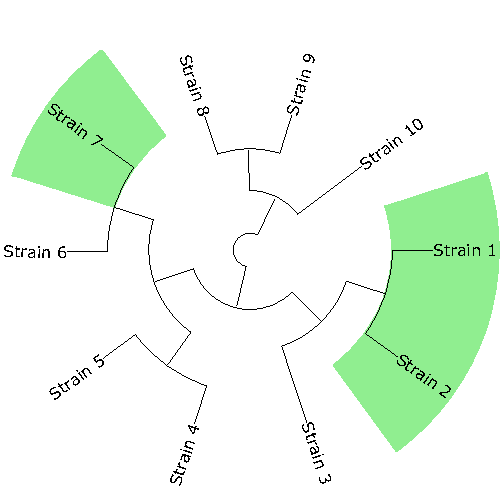
\includegraphics[width=0.9\textwidth]{images/part1/tree_example_1.pdf}
         \caption{Признак с гомоплазией \\(невыпуклый)}
         \label{fig:convex-example-unconvex}
     \end{subfigure}
     \vspace{0.5cm}
     \begin{subfigure}[b]{0.49\textwidth}
         \centering
         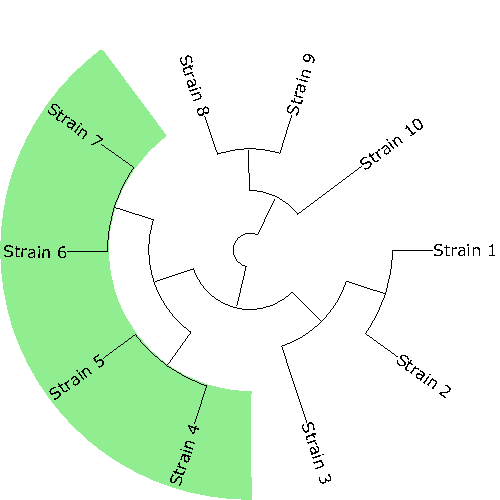
\includegraphics[width=0.9\textwidth]{images/part1/tree_example_2.pdf}
         \caption{Признак, свободный от гомоплазии (выпуклый)}
         \label{fig:convex-example-convex}
     \end{subfigure}
     \caption{Примеры состояния признака на дереве}
     \label{fig:convex-example}
\end{figure}

Более формально: пусть дано множество таксонов $X$ и филогенетическое $X$-дерево $(T, \phi)$, где $T = (V,E)$ — граф, а $\phi: X \rightarrow V$ — отображение, связывающее множество видов с листьями графа.
Признак на множестве таксонов $X$ определяется как функция $\chi$, отображающая некоторое непустое подмножество $X' \subseteq X$ в конечное множество состояний признака $C$:
\[
\chi: X' \rightarrow C.
\]

Признак $\chi$ называется выпуклым на дереве $(T,\phi)$, если существует такая функция расширения признака $\bar{\chi}: V \rightarrow C$, удовлетворяющая следующим условиям:

\begin{enumerate}
    \item $\bar{\chi}(\phi(x)) = \chi(x)$ для всех $x \in X'$, то есть расширение согласовано с исходным распределением признака по листьям;
    \item для каждого состояния признака $\alpha \in C$ индуцированный подграф дерева $T$, образованный вершинами множества $\{ v \in V \mid \bar{\chi}(v) = \alpha \}$, является связным.
\end{enumerate}

Алгоритмически выпуклость признака может быть проверена алгоритмом Фитча.
Этот алгоритм для каждого признака на данном дереве вычисляет минимальное число изменений состояния (0 $\leftrightarrow$ 1, где 1 — признак присутствует) вдоль ветвей, необходимое для воспроизведения наблюдаемого распределения 0/1 на листьях. 
Если минимальное число изменений больше 1, признак не может быть объяснён одним появлением — следовательно, он параллельный.

Важно отметить, что невыпуклость признака может быть следствием как реальных параллельных процессов, так и артефактов (например, неточного построения дерева).
Признак, требующий два изменения, иногда можно сделать выпуклым, чуть изменив топологию дерева.
По этой причине, анализируя параллельные перестройки, следует убедиться в надёжности филогенетической основы и при возможности использовать дополнительные данные (например, информацию о функциях разрываемых регионов), чтобы исключить ложные совпадения.

\subsection{Литературные примеры параллельных изменений}
\label{subsec:parallel_changes_examples}

\begin{figure}[h!]
    \centering
    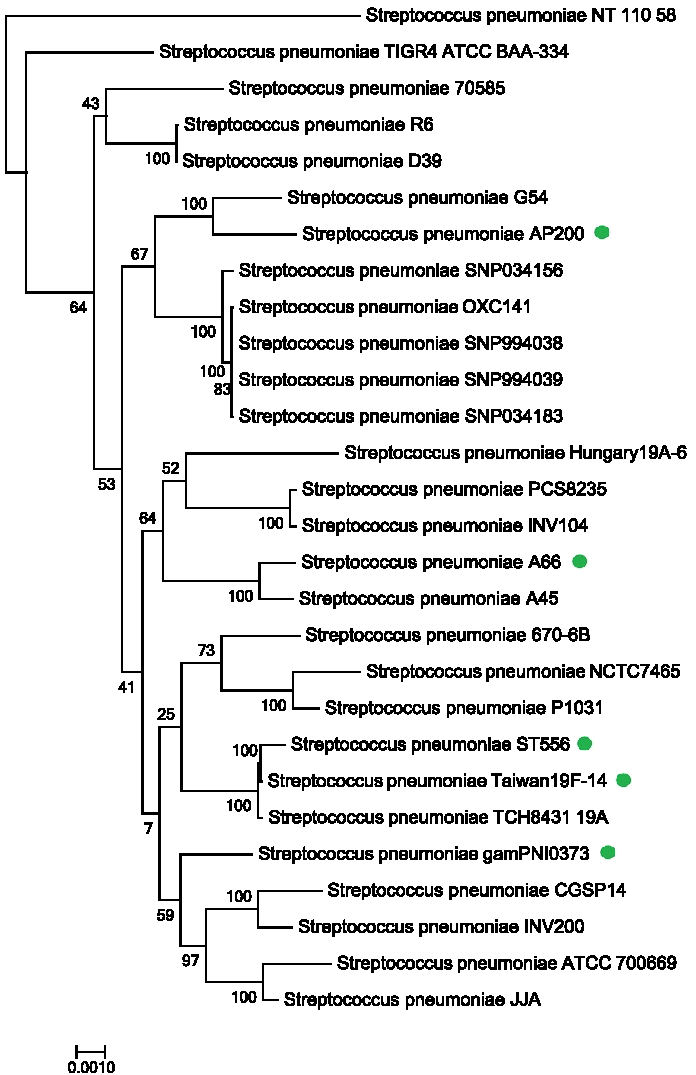
\includegraphics[width=0.55\textwidth]{images/part1/strept-ola-pneu.pdf}
    \caption{Генетическое дерево демонстрирует распределение инверсий по генам PhtD и PhtB, штаммы с такими инверсиями выделены зелёным~\cite{Shelyakin2019}}
    \label{fig:tree-strept}
\end{figure}

Параллельные перестройки геномов наиболее ярко задокументированы у микроорганизмов, где сравнительно небольшие геномы и обилие штаммовых данных позволяют точно отследить независимые события.
Например, в популяциях бактерий \textit{Pseudomonas aeruginosa} наблюдалась инверсия крупного фрагмента хромосомы, фланкированного рибосомными оперонами, которая возникала независимо в разных изолятах~\cite{Irvine2019}.
Показано, что эта перестройка (переворот сегмента между двумя копиями rRNA-гена) приводит к изменениям фенотипа – влиянию на устойчивость к окислительному стрессу, метаболизм и вирулентность; то есть, вероятно, она подвергалась отбору в сходных условиях, возникнув параллельно у разных потомков без недавнего общего предка. 

В работе, посвящённой изучению эволюции стрептококков, выявлены независимые инверсии, связанные с паралогичными генами PhtD и PhtB~\cite{Shelyakin2019}.
Эти перестройки обнаружены у различных штаммов, филогенетически разделённых и не образующих общую кладу по данным генам.
Несмотря на то, что механизм таких инверсий, вероятно, связан с гомологичной рекомбинацией, филогенетический анализ показал, что деревья, построенные на последовательностях генов, задействованных в инверсии, согласуются с общими филогениями этих штаммов, подтверждая независимый характер возникновения событий.
Аналогичные результаты были получены и для других видов рода \textit{Streptococcus}, где параллельные инверсии по указанным паралогам также были выявлены.

Другой пример касается патогенного стрептококка \textit{Streptococcus pyogenes}.
У этого вида обнаружены параллельные изменения числа копий определённых блоков, связанные с фаговыми инсерциями~\cite{Shelyakin2019}.
В частности, блок, содержащий рРНК-оперон, в большинстве геномов представлен несколькими (шестью) копиями, но в некоторых эволюционно удалённых линиях независимо наблюдались либо утраты одной копии, либо, наоборот, приобретение дополнительных копий (до четырёх сверх нормы).
Анализ геномного окружения показал, что эти изменения копийности связаны с независимыми интеграциями и потерями фаговых последовательностей в разных кладах \textit{S.~pyogenes}.
Таким образом, хотя у общего предка всех штаммов было шесть копий оперона, последующие перестройки в различных ветвях привели к разным вариантам — классический случай параллельной эволюции геномной структуры.

Высокие скорости и параллельность перестроек отмечены и в ряде других патогенов.


Хотя большинство исследований параллельных перестроек сосредоточены на прокариотах, аналогичные явления наблюдаются и в эукариотических геномах.
Особенно интересны случаи, в которых крупномасштабные хромосомные инверсии и слияния возникают независимо в различных филогенетических линиях.

Так, в работе~\cite{Porubsky2022} были описаны участки генома человека, демонстрирующие повторяющееся переключение ориентации (англ. \textit{inversion toggling}).
Такие инверсии, возникающие независимо у разных особей, охватывают сотни килобаз и часто обогащены генами.
Интересно, что значительная часть этих регионов совпадает с участками, ранее инвертировавшимися в ходе эволюции приматов, что говорит о древнем и устойчивом характере таких перестроек.

Особый интерес вызывает обнаруженная автором предвзятость по отношению к половым хромосомам: 45\% всех повторяющихся инверсий были локализованы на хромосомах X или Y, что может объясняться особенностями репарации ДНК в непарных участках этих хромосом.
Эти наблюдения подтверждают, что половые хромосомы представляют собой ``горячие точки'' структурной нестабильности, где независимо могут происходить сходные перестройки, включая разрывы и инверсии~\cite{Porubsky2022}.

Стоит отдельно упомянуть гипотезу cети аберрантных филогений, основанная на отборе (англ. \textit{SNAP, Selection-driven Network of Aberrant Phylogenies}), предложенную для объяснения параллельных перестроек~\cite{Brandis2020}.
Согласно этой гипотезе, перестройки могут возникать параллельно под действием сходных селекционных давлений при адаптации к новой нише, особенно если в геноме имеются места, ломкость которых обеспечивает быстрый адаптивный ответ.
Иными словами, сходная среда может ``направлять'' эволюцию разных популяций по похожим структурным путям, вызывая независимые перестройки в аналогичных локусах.
Примеры с инверсиями около rRNA-генов и фаговыми инсерциями в патогенах согласуются с этой идеей, так как соответствующие перестройки дают преимущество в определённых условиях (иммунное уклонение, регуляция вирулентности) и потому появляются в разных линиях независимо.

\subsection{Задача оценки степени параллельности}
\label{subsec:parallelism_estimation}

После выявления параллельных геномных перестроек естественным следующим шагом является количественная оценка степени такого параллелизма.
Понимание, насколько широко распространены независимые повторения структурных изменений, важно для интерпретации их биологического значения и выявления возможных адаптивных механизмов, формирующих эволюцию вида.

В простейшем случае такая оценка может сводиться к подсчёту числа признаков, возникших независимо на разных ветвях филогенетического дерева.
Однако подобный подход не учитывает того, что отдельные события могут повторяться неодинаковое количество раз, и поэтому не всегда отражает истинный масштаб параллельности. 

В связи с этим возникает потребность в более информативных агрегированных показателях, способных учитывать как частоту, так и «силу» повторения перестроек.
Например, таким агрегированным показателем может служить доля параллельных событий от общего числа всех зафиксированных геномных перестроек в данной группе организмов.
Другим примером является индекс гомоплазии, отражающий степень повторности появления одинаковых структурных изменений на эволюционном дереве.
Подобные метрики позволяют дать более глубокое представление о характере и частоте параллельных эволюционных событий и, как следствие, помочь понять их потенциальную адаптивную роль или выявить механизмы структурной нестабильности, присущие определённым геномным регионам.
